\documentclass{standalone}
\usepackage{tikz,ctex}
\usepackage{tikz-3dplot} % 2-1
\usepackage{unicode-math} % 2-5,4-1,4-2
\setmathfont{Fira Math Regular}
\setmainfont{Fira Sans}
\definecolor{background}{RGB}{239, 239, 239} % 4-5,6-2,6-5
\begin{document}
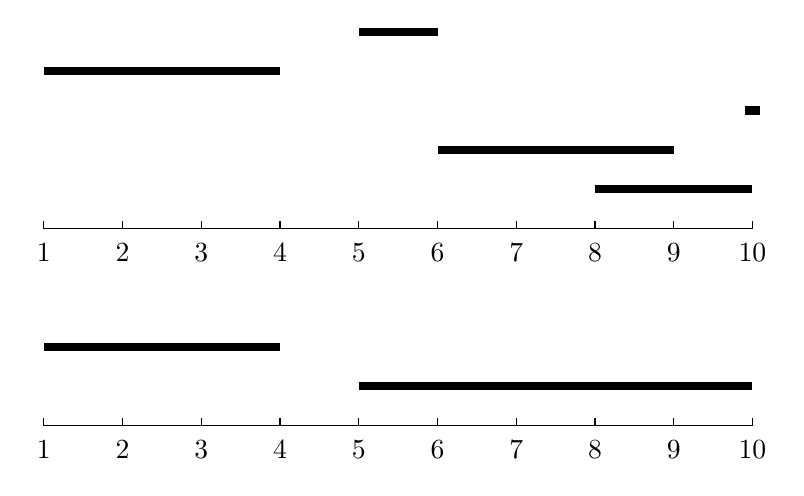
\begin{tikzpicture}
\foreach \x/\y/\i in{5/6/1,1/5.5/3,9.9/5/.2,6/4.5/3,8/4/2,1/2/3,5/1.5/5}{
    \draw[line width=3pt] (\x,\y) --(\x+\i,\y);}
\foreach \x in {1,...,10}
\foreach \y in{1,3.5}{
    \draw (\x,\y)--(\x,\y+.1);
    \node at (\x,\y-.3){\x};}
\draw (1,1)--(10,1);
\draw (1,3.5)--(10,3.5);
\end{tikzpicture}
\end{document}